\documentclass[0_en]{subfiles}

\begin{document}

\section{Quasi-Newton Methods}\label{sec:background_quasi_newton}

\begin{figure}[t]
    \centering
    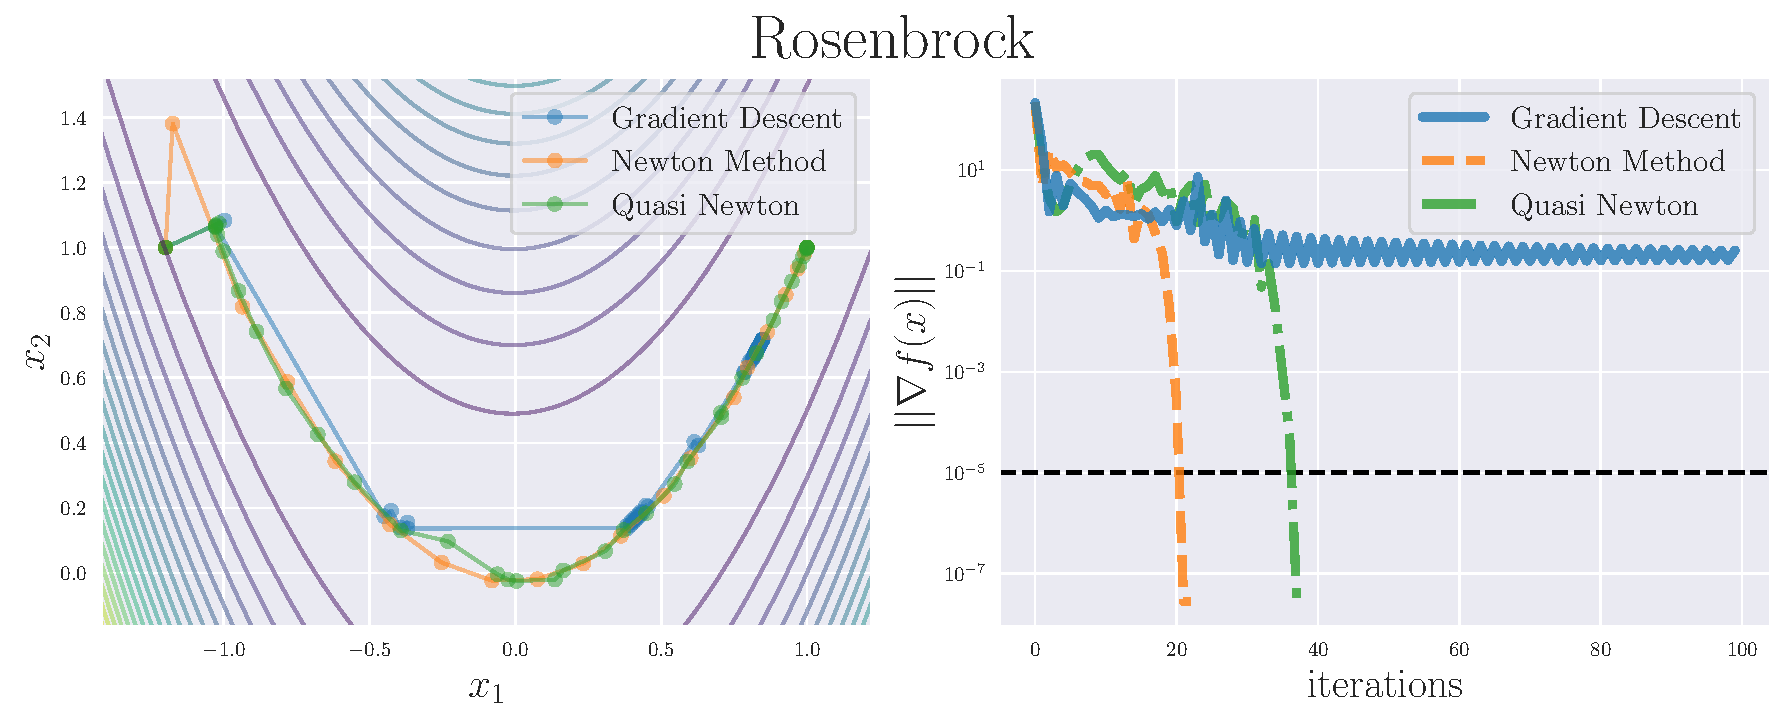
\includegraphics[width=\textwidth]{../imgs/quasi_newton/newton_vs_qs_vs_gd.pdf}
    \caption{Comparison of Newton's method, quasi-Newton methods, and gradient descent}
    \label{fig:newton_vs_qs_vs_gd}
\end{figure}

In this section, we discuss quasi-Newton methods. Quasi-Newton methods are based on Newton's method, but aim to reduce its primary drawback, namely, the high computational cost of evaluating the Hessian matrix. Specifically, instead of using the true Hessian matrix $\nabla^2 f(x_k)$, an approximation matrix $B_k$ is employed, thereby achieving fast convergence while keeping the computational cost low.

\Cref{fig:newton_vs_qs_vs_gd} shows a comparison of Newton's method, quasi-Newton methods, and gradient descent. Gradient descent is a method that simply updates in the direction opposite to the gradient. Although its per-iteration computational cost is the lowest, its convergence is slow. Newton's method converges in the fewest iterations, but has the highest computational cost per step. Quasi-Newton methods lie between these two extremes, striking a balance between them. In particular, when comparing methods in terms of computation time rather than the number of iterations, quasi-Newton methods often exhibit the best performance.

Line-search-based quasi-Newton methods generate a sequence $\{ x_k \}_{k=0}^{\infty}$ converging to the optimal solution $x^*$ as follows:
\begin{equation*}
    x_{k+1} = x_k - \alpha_k B_k^{-1} \nabla f(x_k)
    = x_k - \alpha_k H_k \nabla f(x_k)
\end{equation*}
Here, $\alpha_k > 0$ is the step size determined by line search, $B_k$ is an approximation of the Hessian matrix $\nabla^2 f(x_k)$ at the point $x_k$, and $H_k \coloneqq B_k^{-1}$ denotes its inverse.

\begin{figure}[t]
    \begin{minipage}{0.33\textwidth}
        \centering
        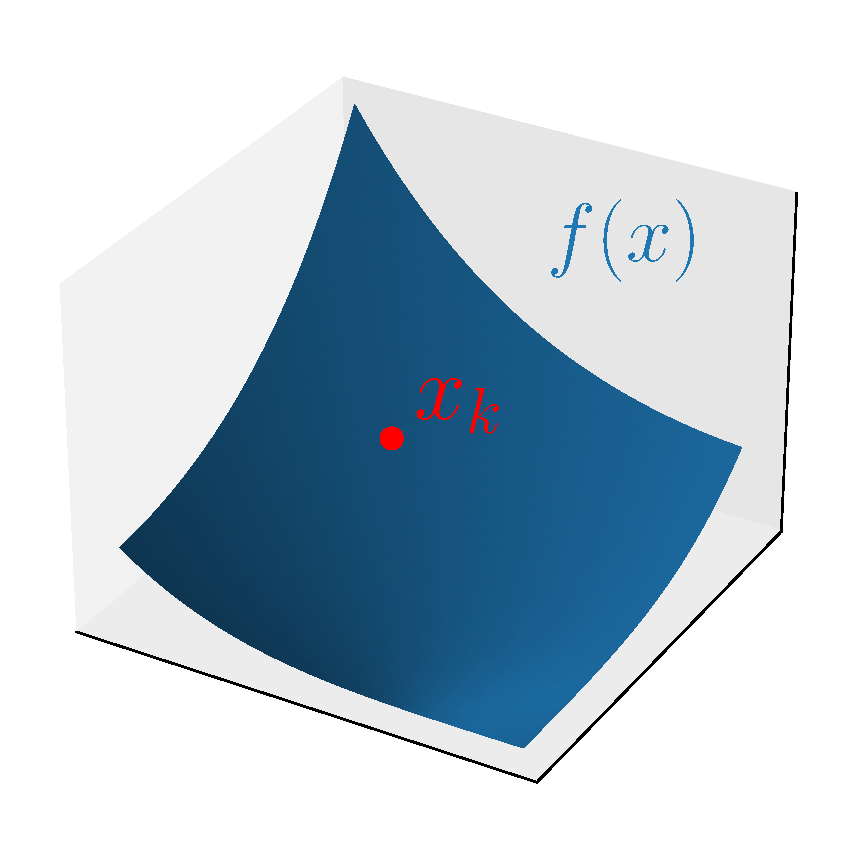
\includegraphics[width=\textwidth]{../imgs/quasi_newton/quasi_newton_1.pdf}
    \end{minipage}%
    \begin{minipage}{0.33\textwidth}
        \centering
        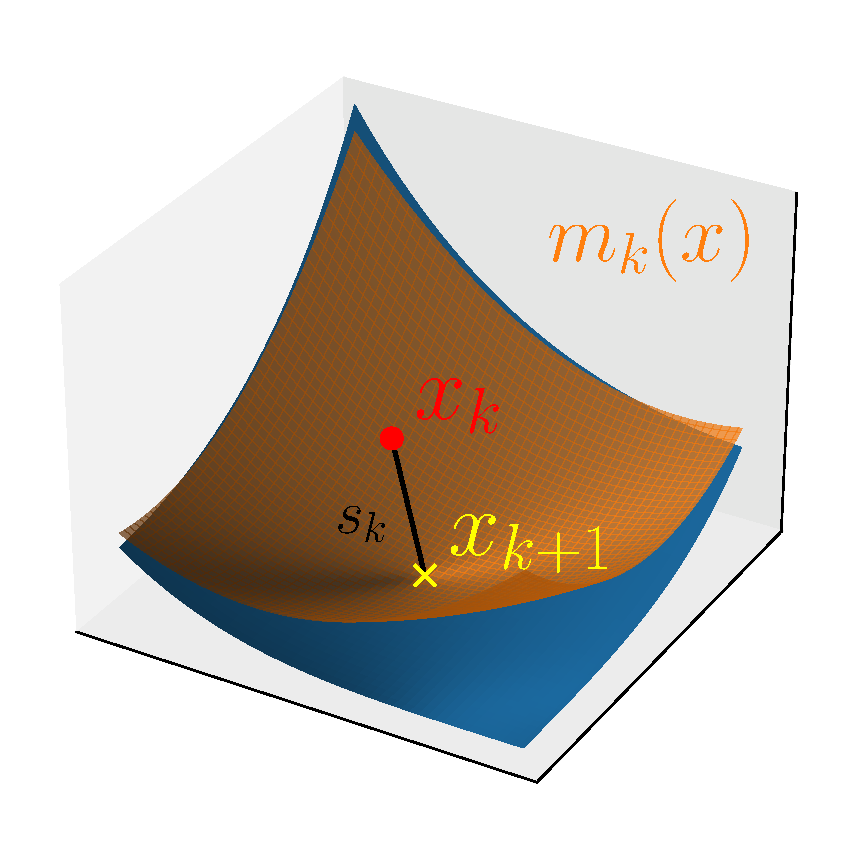
\includegraphics[width=\textwidth]{../imgs/quasi_newton/quasi_newton_2.pdf}
    \end{minipage}%
    \begin{minipage}{0.33\textwidth}
        \centering
        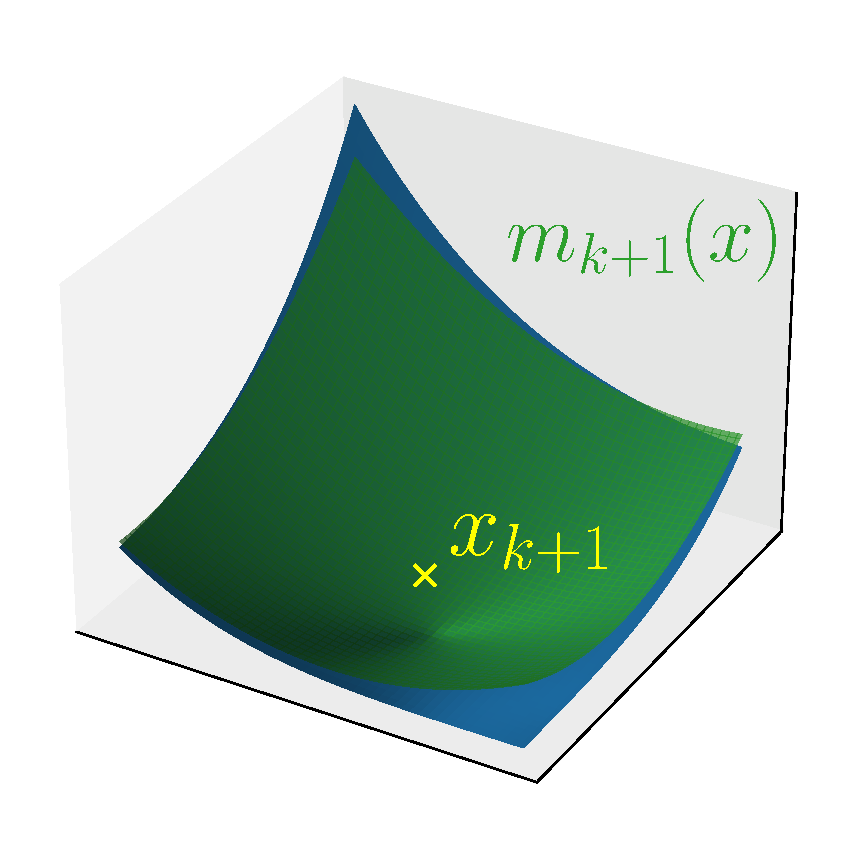
\includegraphics[width=\textwidth]{../imgs/quasi_newton/quasi_newton_3.pdf}
    \end{minipage}
    \caption{
        Conceptual illustration of quasi-Newton methods.
        (1) The objective function $f$ (blue surface) and the current point $x_k$ (red dot).
        (2) The quadratic model induced by the current Hessian approximation (orange surface) and its minimizer $x_{k+1}$ (yellow cross).
        (3) The updated quadratic model based on the new point $x_{k+1}$ (green surface).
    }
    \label{fig:quasi_newton_overview}
\end{figure}

The core of quasi-Newton methods lies in how to update $B_k$ (or its inverse $H_k$) at each iteration so that it approaches the Hessian matrix $\nabla^2 f(x_k)$. \Cref{fig:quasi_newton_overview} illustrates this concept. First, around the current point $x_k$, a quadratic approximation model of the objective function $f$ is constructed using $B_k$. Next, this quadratic model is minimized to obtain the next point $x_{k+1}$. After obtaining $x_{k+1}$, the approximation matrix $B_k$ is updated to $B_{k+1}$ using the gradient information at $x_k$ and $x_{k+1}$. This procedure is repeated until convergence, which constitutes the quasi-Newton method.

In what follows, we introduce the secant condition that the approximate Hessian matrix $B_k$ is required to satisfy, and present several representative update formulas for such $B_k$ and $H_k$.

\subsection{Secant Condition}

In this section as well, let $f\colon \mathbb{R}^n \to \mathbb{R}$ be of class $C^2$.
Suppose that a symmetric matrix $B_k$ is given as an approximation of the Hessian matrix $\nabla^2 f(x_k)$.
We determine an approximation Hessian $B_{k+1}$ at the next point $x_{k+1}$.
Although there are infinitely many possible candidates for such a matrix, it is natural to impose symmetry on $B_{k+1}$ as well, given that the true Hessian matrix is symmetric.
Define the step and gradient difference as
\begin{equation*}
    s_k = x_{k+1} - x_k, \qquad   y_k = \nabla f(x_{k+1}) - \nabla f(x_k),
\end{equation*}
where we assume that $y_k^\top s_k \neq 0$ and $s_k \neq 0$. Here, the $s$ in $s_k$ stands for step.
Using the Taylor expansion of $\nabla f(x_k)$, we have
\begin{align*}
    \nabla f(x_k) & = \nabla f(x_{k+1}) + \nabla^2 f(x_{k+1})(x_k - x_{k+1}) + \order{\norm{x_k - x_{k+1}}^2} \\
                  & \approx \nabla f(x_{k+1}) + \nabla^2 f(x_{k+1})(x_k - x_{k+1})                            \\
                  & \approx \nabla f(x_{k+1}) + B_{k+1}(x_k - x_{k+1})
\end{align*}
Requiring the above approximation to hold as an equality yields
\begin{equation*}
    B_{k+1}(x_{k+1} - x_k) = \nabla f(x_{k+1}) - \nabla f(x_k),
\end{equation*}
or equivalently,
\begin{equation}\label{eq:secant-condition}
    B_{k+1} s_k = y_k.
\end{equation}
The relation in \cref{eq:secant-condition} is called the secant condition, or the quasi-Newton equation.

\subsection{Representative Quasi-Newton Update Rules}

Given $B_k$, $s_k$, and $y_k$, there exist many update rules that produce $B_{k+1}$ satisfying the secant condition. We introduce several representative ones with their derivations \citep{dennisjr.QuasiNewtonMethodsMotivation1977a}.
In this subsection only, for brevity, we abbreviate $B_k$, $B_{k+1}$, $s_k$, and $y_k$ as $B$, $\bar{B}$, $s$, and $y$, respectively.

\subsubsection{Broyden's Update}
% https://en.wikipedia.org/wiki/Broyden%27s_method

Broyden's update is one of the most fundamental quasi-Newton update formulas, but it is not popular in practice due to its lack of symmetry preservation.
The update formulas are given by
\begin{align}
    \bar{B}_{\mathrm{Broyden}} & = B + \frac{(y - Bs)s^\top}{s^\top s}, \label{eq:broyden-update}           \\
    \bar{H}_{\mathrm{Broyden}} & = H + \frac{s - Hy}{s^\top Hy} s^\top H. \label{eq:broyden-inverse-update}
\end{align}

\paragraph{Derivation}

We derive this formula from simple structural assumptions \citep[Section 4]{dennisjr.QuasiNewtonMethodsMotivation1977a}.
\begin{proposition}
    Assume that $\bar{B}$ satisfies the secant condition
    \begin{equation}\label{eq:secant-broyden}
        \bar{B}s = y,
    \end{equation}
    and the action constraint
    \begin{equation}\label{eq:action-constraint}
        \bar{B}z = Bz
        \quad\text{for all } z\in\mathbb{R}^n \text{ such that } z^\top s = 0.
    \end{equation}
    Then $\bar{B}$ is uniquely determined and it is $\bar{B}_{\mathrm{Broyden}}$ defined by \cref{eq:broyden-update}.
\end{proposition}
\begin{proof}
    A basis for $\mathbb{R}^n$ can be constructed from $s$ and a basis for the orthogonal complement of $s$. Since \cref{eq:secant-broyden,eq:action-constraint} completely determine the action of $\bar{B}$ with respect to this basis, $\bar{B}$ is uniquely determined.

    We now show that $\bar{B}_{\mathrm{Broyden}}$ defined by \cref{eq:broyden-update} satisfies \cref{eq:secant-broyden,eq:action-constraint}. Let $z$ be any vector satisfying $z^\top s = 0$. Then
    \begin{align*}
        \bar{B}_{\mathrm{Broyden}} s
         & = \qty(B + \frac{(y - Bs)s^\top}{s^\top s}) s
        = Bs + (y - Bs)
        = y,                                             \\
        \bar{B}_{\mathrm{Broyden}} z
         & = \qty(B + \frac{(y - Bs)s^\top}{s^\top s}) z
        = Bz + (z^\top s) \frac{y - Bs}{s^\top s}
        = Bz.
    \end{align*}
    Hence $\bar{B}_{\mathrm{Broyden}}$ indeed satisfies \cref{eq:secant-broyden,eq:action-constraint}. Therefore, by uniqueness, we have $\bar{B} = \bar{B}_{\mathrm{Broyden}}$.
\end{proof}

Broyden's update can also be characterized as a minimal-change update in the Frobenius norm.

\begin{proposition}[\citep{dennisjr.QuasiNewtonMethodsMotivation1977a}, Theorem~4.1]
    Let $B\in\mathbb{R}^{n\times n}$, $y\in\mathbb{R}^n$, and $s\in\mathbb{R}^n\setminus\{0\}$ be given.
    Then the matrix $\bar{B}$ defined by \cref{eq:broyden-update} is the unique solution of
    \begin{mini*}
        {\tilde{B} \in \mathbb{R}^{n \times n}}
        {\norm{\tilde{B} - B}_F}
        {}
        {\label{eq:broyden-minimal-change}}
        \addConstraint{\tilde{B} s}{= y.}
    \end{mini*}
\end{proposition}
\begin{proof}
    The function $\tilde{B}\mapsto\norm{\tilde{B}-B}_F$ is strictly convex on $\mathbb{R}^{n\times n}$.
    The constraint set
    \begin{equation}
        \{\tilde{B}\in\mathbb{R}^{n\times n}:\tilde{B}s=y\}
    \end{equation}
    is affine and hence convex.
    Therefore, the optimization problem admits at most one minimizer.

    To show that $\bar{B}=\bar{B}_{\mathrm{Broyden}}$ defined by \cref{eq:broyden-update} is indeed the minimizer, we compute:
    \begin{equation*}
        \norm{\bar{B}_{\mathrm{Broyden}} - B}_F^2
        = \norm{\frac{(y-Bs)s^\top}{s^\top s}}_F^2
        = \norm{(\tilde{B}-B) \frac{s s^\top}{s^\top s}}_F^2
        \leq \norm{\tilde{B}-B}_F^2,
    \end{equation*}
    where we used the sub-multiplicativity of Frobenius norm and the fact that $\norm{ss^\top/(s^\top s)}_F=1$ in the last inequality.
    Thus, $\tilde{B}=\bar{B}_{\mathrm{Broyden}}$.
\end{proof}

Broyden's update is characterized by two properties: it satisfies the secant condition and preserves the action on vectors orthogonal to $s$. Additionally, it is the unique minimal-change update in the Frobenius norm subject to the secant constraint.

\subsubsection{SR1 Update}
% https://en.wikipedia.org/wiki/Symmetric_rank-one

The Symmetric Rank-One (SR1) update \citep{nocedal1999numerical} is a fundamental quasi-Newton method that maintains symmetry throughout the update process. The update formulas are given by
\begin{align}
    \bar{B}_{\mathrm{SR1}} & = B + \frac{(y - B s)(y - B s)^\top}{(y - B s)^\top s}, \label{eq:sr1-b-update} \\
    \bar{H}_{\mathrm{SR1}} & = H + \frac{(s - H y)(s - H y)^\top}{(s - H y)^\top y}. \label{eq:sr1-h-update}
\end{align}

\paragraph{Derivation}

To derive \cref{eq:sr1-b-update}, we construct the updated matrix $\bar{B}$ as a rank-one update. That is, we assume that for some vector $z \in \mathbb{R}^n$,
\begin{equation}\label{eq:sr1-symmetric-form}
    \bar{B}_{\mathrm{SR1}} = B + z z^\top.
\end{equation}
For this update to satisfy the secant condition $\bar{B}_{\mathrm{SR1}} s = y$, assuming $z^\top s \neq 0$, we require
\begin{equation}\label{eq:sr1-secant-condition}
    B s + z z^\top s = y,
\end{equation}
which yields
\begin{equation}\label{eq:sr1-z-formula}
    z = \frac{y - B s}{z^\top s}.
\end{equation}

To determine $z^\top s$, we take the inner product of both sides of \cref{eq:sr1-z-formula} with $s$:
\begin{equation}\label{eq:sr1-self-consistency}
    z^\top s = \frac{(y - B s)^\top s}{z^\top s}.
\end{equation}
Rearranging \cref{eq:sr1-self-consistency} yields the key relation
\begin{equation}\label{eq:sr1-zs-squared}
    (z^\top s)^2 = (y - B s)^\top s.
\end{equation}

Substituting \cref{eq:sr1-zs-squared} into \cref{eq:sr1-z-formula} and using \cref{eq:sr1-symmetric-form}, we obtain
\begin{align}\label{eq:sr1-derivation-final}
    \bar{B}_{\mathrm{SR1}}
     & = B + z z^\top                                          \\
     & = B + \frac{(y - B s)(y - B s)^\top}{(z^\top s)^2}      \\
     & = B + \frac{(y - B s)(y - B s)^\top}{(y - B s)^\top s},
\end{align}
which is the SR1 update formula stated in \cref{eq:sr1-b-update}.

\paragraph{Remarks}

The SR1 update requires $(y - Bs)^\top s \neq 0$ to be well-defined. When $(y - Bs)^\top s = 0$, the denominator in \cref{eq:sr1-b-update} vanishes, and the update is typically skipped in practice. This situation can occur when the secant condition cannot be satisfied by a symmetric rank-one update, indicating that more sophisticated update strategies are needed.

\subsubsection{Powell Symmetric Broyden (PSB) Update}

The Powell Symmetric Broyden (PSB) update \cite{haeltermanAnalyticalStudyLeast2009} is one of the most important quasi-Newton update rules. The update formulas are given by
\begin{align}
    \bar{B}_{\mathrm{PSB}} & = B + \frac{(y - B s) s^\top + s (y - B s)^\top}{s^\top s} - \frac{s^\top (y - B s)}{(s^\top s)^2} s s^\top, \label{eq:psb-b-update} \\
    \bar{H}_{\mathrm{PSB}} & = H + \frac{(s - H y) y^\top + y (s - H y)^\top}{y^\top y} - \frac{y^\top (s - H y)}{(y^\top y)^2} y y^\top. \label{eq:psb-h-update}
\end{align}

\paragraph{Derivation}

To understand the motivation behind this formula, we note that in the SR1 update, the rank-one update was formulated symmetrically as $\bar{B}_{\mathrm{SR1}} = B + z z^\top$.
We may relax the requirement of maintaining symmetry throughout the update process. Instead, we can consider an asymmetric rank-one update of the form $z c^\top$, where the final result is symmetrized afterward.

For a given vector $c \in \mathbb{R}^n$ with $c^\top s \neq 0$, we define
\begin{equation}\label{eq:z-definition}
    z = \frac{y - B s}{c^\top s}
\end{equation}
and perform the asymmetric update
\begin{equation}\label{eq:asymmetric-update}
    C_1 \coloneqq B + \frac{(y - B s)c^\top}{c^\top s}.
\end{equation}
Since $C_1$ is generally not symmetric, we symmetrize it via
\begin{equation}\label{eq:symmetrization}
    C_2 = \frac{C_1 + C_1^\top}{2}.
\end{equation}
However, the symmetrized matrix $C_2$ may not satisfy the secant condition $C_2 s = y$. Therefore, we iterate this process:
\begin{equation}\label{eq:psb-iteration}
    \begin{dcases}
        C_0 = B                                                                               \\
        C_{2t+1} = C_{2t} + \frac{(y - C_{2t}s)c^\top}{c^\top s} & \text{(asymmetric update)} \\
        C_{2t+2} = \frac{C_{2t+1} + C_{2t+1}^\top}{2}            & \text{(symmetrization)}
    \end{dcases}
\end{equation}

The key result is that the sequence $\{ C_{2t} \}_{t=0}^{\infty}$ converges to a symmetric matrix satisfying the secant condition, as formalized in the following proposition.

\begin{proposition}[\citep{dennisjr.QuasiNewtonMethodsMotivation1977a}, Lemma~7.2]\label{prop:psb-convergence}
    The sequence $\{ C_{2t} \}_{t=0}^{\infty}$ defined by \cref{eq:psb-iteration} converges, and the limit is given by
    \begin{equation}\label{eq:psb-limit}
        \lim_{t \to \infty} C_{2t}
        = B + \frac{(y - Bs)c^\top + c(y - Bs)^\top}{c^\top s} - \frac{(y - Bs)^\top s}{(c^\top s)^2} c c^\top.
    \end{equation}
\end{proposition}
\begin{proof}
    We first analyze the even subsequence.
    Define
    \begin{equation*}
        G_k \coloneqq C_{2k}
    \end{equation*}
    for $k=0,1,2,\dots$.
    By construction, each $G_k$ is symmetric.
    From \cref{eq:psb-iteration} and the definition, we have
    \begin{equation*}
        G_{k+1} = G_k +\frac{1}{2c^\top s}\qty((y-G_k s)c^\top+c(y-G_k s)^\top).
    \end{equation*}
    Let us introduce the error vector
    \begin{equation}\label{eq:wk-definition}
        w_k \coloneqq y-G_k s
    \end{equation}
    and then we have
    \begin{equation}\label{eq:Gupdate}
        G_{k+1} = G_k+\frac{1}{2c^\top s}(w_k c^\top+cw_k^\top).
    \end{equation}
    Substituting \cref{eq:Gupdate} into \cref{eq:wk-definition} yields
    \begin{align}
        w_{k+1} & = y-\qty(G_k+\frac{1}{2c^\top s}(w_k c^\top+cw_k^\top))s \\
                & =
        w_k-\frac12w_k-\frac{w_k^\top s}{2c^\top s}c                       \\
                & =
        \frac{1}{2}\qty(w_k-\frac{w_k^\top s}{c^\top s}c).
    \end{align}
    Hence
    \begin{equation}
        w_{k+1}=Pw_k,
        \qquad
        P \coloneqq \frac{1}{2}\left(I-\frac{cs^\top}{c^\top s}\right).
    \end{equation}
    The matrix $cs^\top/c^\top s$ has rank one and eigenvalues $1,0,\dots,0$.
    Therefore, $P$ has one eigenvalue $0$ and all remaining eigenvalues equal to $1/2$.
    In particular, its spectral radius is $1/2<1$.
    Thus, the Neumann series converges and
    \begin{align}
        \sum_{k=0}^{\infty}w_k & =        \sum_{k=0}^{\infty}P^k(y-Bs)                  &  & (\text{from } w_0=y-Bs)                               \\
                               & =  (I-P)^{-1}(y-Bs)                                                                                               \\
                               & = 2\qty(I-\frac{1}{2}\frac{cs^\top}{c^\top s}) (y-Bs). &  & (\text{from the definition of } P) \label{eq:wseries}
    \end{align}
    Note that the last equation follows from
    \begin{equation*}
        2(I-P) \qty(I-\frac{1}{2}\frac{cs^\top}{c^\top s}) = \qty(I + \frac{cs^\top}{c^\top s}) \qty(I-\frac{1}{2}\frac{cs^\top}{c^\top s}) = I.
    \end{equation*}
    In particular, $\norm{w_k}\to0$ as $k\to\infty$.
    Hence, from \cref{eq:Gupdate}, we have
    \begin{align}
        \lim_{k\to\infty}G_k
         & =
        B+\frac{1}{2c^\top s}
        \sum_{k=0}^{\infty}(w_k c^\top+c w_k^\top)                                                                                     \\
         & = B+ \qty(\sum_{k=0}^{\infty}w_k) \frac{c^\top}{2c^\top s} + \frac{c}{2c^\top s} \qty(\sum_{k=0}^{\infty}w_k)^\top          \\
         & = B + \frac{(y - Bs)c^\top + c(y - Bs)^\top}{c^\top s} - \frac{(y - Bs)^\top s}{(c^\top s)^2} c c^\top.  \label{eq:G-limit}
    \end{align}
    Thus $G_k\to\bar B$.
    Finally,
    \begin{equation}
        C_{2k+1}
        =
        G_k+\frac{w_k c^\top}{c^\top s}.
    \end{equation}
    Since $G_k\to\bar B$ and $\norm{w_k}\to0$, we obtain
    \begin{equation}
        C_{2k+1}-G_k\to0.
    \end{equation}
    Therefore both subsequences $\{C_{2k}\}$ and $\{C_{2k+1}\}$ converge to $\bar B$,
    and hence
    \begin{equation}
        C_k\to\bar B.
    \end{equation}
    This completes the proof.
\end{proof}

\noindent When $c = s$, the general formula in \cref{eq:psb-limit} simplifies to the standard PSB update formula:
\begin{equation}\label{eq:psb-standard}
    \bar{B}_{\mathrm{PSB}} = B + \frac{(y - Bs)s^\top + s(y - Bs)^\top}{s^\top s} - \frac{(y - Bs)^\top s}{(s^\top s)^2} ss^\top,
\end{equation}
which matches \cref{eq:psb-b-update}.

\paragraph{Remarks}

The choice of $c = s$ is motivated by ensuring positive definiteness of the resulting update. The PSB update can be viewed as the limit of an iterative symmetrization process applied to asymmetric rank-one updates.

\subsubsection{DFP Update}
% https://en.wikipedia.org/wiki/Davidon%E2%80%93Fletcher%E2%80%93Powell_formula

The Davidon--Fletcher--Powell (DFP) update \cite{nocedal1999numerical} is a classical quasi-Newton update formula. The update formulas are given by
\begin{align}
    \bar{B}_{\mathrm{DFP}} & = (I - \frac{y s^\top}{y^\top s}) B (I - \frac{s y^\top}{y^\top s}) + \frac{y y^\top}{y^\top s}, \label{eq:dfp-b-update} \\
    \bar{H}_{\mathrm{DFP}} & = H - \frac{H y y^\top H}{y^\top H y} + \frac{s s^\top}{y^\top s}. \label{eq:dfp-h-update}
\end{align}

\paragraph{Derivation}

In the PSB update rule discussed earlier, we substituted $c=s$, but we can consider taking a different $c$. Specifically, we consider choosing $c$ such that $B_{k+1}$ becomes positive definite. Substituting $c=y$ yields the alternative form:
\begin{equation}\label{eq:dfp-b-alternative}
    \bar{B}_{\mathrm{DFP}} = B + \frac{(y - Bs)y^\top + y(y - Bs)^\top}{y^\top s} - \frac{(y - Bs)^\top s}{(y^\top s)^2} yy^\top.
\end{equation}

% Cauchy's Interlacing Theoremの亜種として知られているようです。

% https://simple-complexities.github.io/eigenvalue/interlacing/2020/02/10/interlacing.html

\subsubsection{BFGS Update}
% https://en.wikipedia.org/wiki/Broyden%E2%80%93Fletcher%E2%80%93Goldfarb%E2%80%93Shanno_algorithm

The Broyden--Fletcher--Goldfarb--Shanno (BFGS) update is one of the most widely used quasi-Newton methods. The update formulas are given by
\begin{align}
    \bar{B}_{\mathrm{BFGS}} & = B - \frac{B s s^\top B}{s^\top B s} + \frac{y y^\top}{y^\top s}, \label{eq:bfgs-b-update-brief}                                       \\
    \bar{H}_{\mathrm{BFGS}} & = \qty(I - \frac{s y^\top}{y^\top s}) H \qty(I - \frac{y s^\top}{y^\top s}) + \frac{s s^\top}{y^\top s}. \label{eq:bfgs-h-update-brief}
\end{align}

\paragraph{Derivation}

This update can be derived by considering the dual of the DFP update. Specifically, we seek an update that minimizes the change in the inverse Hessian approximation $H$ while satisfying the secant condition. Further details are provided in the following subsection.

\subsection{BFGS Method}

In this subsection, we focus on the BFGS update and provide a detailed derivation of its formula.
BFGS update is known as one of the most successful quasi-Newton update rules in practice.
Recall that the BFGS update formula is given by
\begin{equation}
    B_{k+1}   = B_k - \frac{B_k s_k s_k^\top B_k}{s_k^\top B_k s_k} + \frac{y_k y_k^\top}{y_k^\top s_k}. \label{eq:Bk_rank}
\end{equation}

\subsubsection{Formula for \texorpdfstring{$H_k$}{Hk}}

The inverse of the BFGS update $H_k \coloneqq B_k^{-1}$ is given by
\begin{equation}
    H_{k+1} = \qty(I - \frac{s_k y_k^\top}{y_k^\top s_k}) H_k \qty(I - \frac{y_k s_k^\top}{y_k^\top s_k}) + \frac{s_k s_k^\top}{y_k^\top s_k}. \label{eq:Hk_rank}
\end{equation}
We now prove that \cref{eq:Hk_rank} indeed gives the inverse of the BFGS update.

\begin{proposition}
    \Cref{eq:Hk_rank} gives the exact inverse of the BFGS update, i.e., $H_{k+1} = B_{k+1}^{-1}$.
\end{proposition}
\begin{proof}
    The BFGS update can be rewritten in a compact rank-two form
    \begin{equation}\label{eq:bfgs-ucv}
        B_{k+1} = B_k + UCV^\top
    \end{equation}
    where
    \begin{equation*}
        U = \mqty[B_k s_k & y_k],\qquad
        C = \mqty(-\frac{1}{s_k^\top B_k s_k} & 0 \\ 0 & \frac{1}{y_k^\top s_k}),\qquad
        V = \mqty[B_k s_k & y_k]
    \end{equation*}
    since
    \begin{equation}
        U C V^\top   = \mqty[ -\frac{B_k s_k}{s_k^\top B_k s_k}&    \frac{y_k}{y_k^\top s_k} ] \mqty[ s_k^\top B_k  \\  y_k^\top ]
        = -\frac{B_k s_k s_k^\top B_k}{s_k^\top B_k s_k} + \frac{y_k y_k^\top}{y_k^\top s_k}.
    \end{equation}
    By the Sherman--Morrison--Woodbury identity, we have
    \begin{align*}
        H_{k+1} & = (B_k + U C V^\top)^{-1}                                                                                                                                                                                                                    \\
                & = B_k^{-1}- B_k^{-1}U\qty(C^{-1}+V^\top B_k^{-1}U)^{-1}V^\top B_k^{-1}                                                                                                                                                                       \\
                & = H_k- \mqty[s_k                                                                                                                             & H_k y_k]\qty(\mqty(- s_k^\top B_k s_k                                         & 0             \\0    & y_k^\top s_k)+\mqty(s_k^\top B_k s_k   & s_k^\top y_k      \\y_k^\top s_k & y_k^\top H_k y_k))^{-1}\mqty[s_k^\top   \\ y_k^\top H_k] \\
                & = H_k- \mqty[s_k                                                                                                                             & H_k y_k]\mqty(0                                                               & y_k^\top s_k  \\y_k^\top s_k       & y_k^\top H_k y_k + y_k^\top s_k)^{-1}\mqty[s_k^\top                         \\     y_k^\top H_k]                 \\
                & = H_k- \mqty[s_k                                                                                                                             & H_k y_k]\qty(-\frac{1}{(y_k^\top s_k)^2}\mqty(y_k^\top H_k y_k + y_k^\top s_k & -y_k^\top s_k \\-y_k^\top s_k                 & 0    )) \mqty[ s_k^\top                                                      \\     y_k^\top H_k]  \\
                & = H_k+\frac{1}{(y_k^\top s_k)^2}\mqty[s_k                                                                                                    & H_k y_k] \mqty(y_k^\top H_k y_k + y_k^\top s_k                                & -y_k^\top s_k \\-y_k^\top s_k                 & 0) \mqty[s_k^\top                                                             \\    y_k^\top H_k]\\
                & = H_k+\frac{1}{(y_k^\top s_k)^2} \qty((y_k^\top H_k y_k + y_k^\top s_k) s_k s_k^\top - (y_k^\top s_k)(s_k y_k^\top H_k + H_k y_k s_k^\top) )                                                                                                 \\
                & = \qty(I - \frac{s_k y_k^\top}{y_k^\top s_k}) H_k \qty(I - \frac{y_k s_k^\top}{y_k^\top s_k}) + \frac{s_k s_k^\top}{y_k^\top s_k}.
    \end{align*}
    which completes the proof.
\end{proof}

\subsubsection{Positive Definiteness of \texorpdfstring{$B_{k+1}$}{Bk+1}}

An important property of the BFGS update is that if the current approximation $B_k$ is positive definite and the curvature condition $y_k^\top s_k > 0$ holds, then the updated approximation $B_{k+1}$ is also guaranteed to be positive definite.

\begin{proposition}
    If $B_k$ is positive definite and $y_k^\top s_k > 0$, then $B_{k+1}$ defined by \cref{eq:Bk_rank} is also positive definite.
\end{proposition}
\begin{proof}
    By assumption, $B_k$ and its inverse $H_k$ are positive definite.
    For any nonzero vector $v \in \mathbb{R}^n$, we have
    \begin{align*}
        v^\top H_{k+1} v
         & = v^\top \qty(I - \frac{s_k y_k^\top}{y_k^\top s_k}) H_k \qty(I - \frac{y_k s_k^\top}{y_k^\top s_k}) v + v^\top \frac{s_k s_k^\top}{y_k^\top s_k} v \\
         & \geq 0 + \frac{(s_k^\top v)^2}{y_k^\top s_k} > 0,
    \end{align*}
    where the first term is nonnegative since $H_k$ is positive definite, and the second term is positive due to the curvature condition $y_k^\top s_k > 0$.
    Thus, $H_{k+1}$ is positive definite, and consequently, $B_{k+1} = H_{k+1}^{-1}$ is also positive definite.
\end{proof}

\subsubsection{KL}

We next present a variational characterization of the BFGS update via the Kullback--Leibler (KL) divergence.
For zero-mean multivariate Gaussians $\mathcal{N}(0,A^{-1})$ and $\mathcal{N}(0,B^{-1})$, the expression
\begin{equation*}
    \psi(A) = \operatorname{tr}(A) - \log \det(A)
\end{equation*}
coincides with the KL divergence up to the additive constant $-n$, so minimizing $\psi$ is equivalent to minimizing the KL distance.
Then, the BFGS update is given by the solution to the optimization problem
\begin{mini*}
    {B \in \mathrm{PD}(n)}
    {\psi(B_k^{-1/2} B B_k^{-1/2})}
    {\label{eq:bfgs-kl}}{}
    \addConstraint{Bs_k}{= y_k}
\end{mini*}
The constraint $B s_k = y_k$ in the optimization problem is precisely the secant condition discussed earlier, ensuring that the updated matrix interpolates the latest curvature pair.

% todo: prove

See literature for proof of these formulations \citep{kanamoriBregmanExtensionQuasiNewton2010,kanamoriBregmanExtensionQuasiNewton2010a}
% (see also \href{http://matsuzoe.web.nitech.ac.jp/infogeo/OCAMI2010/kanamori.pdf}{Japanese slide}).

\subsubsection{Trace and Determinant Formulas for the BFGS Update}

We also present trace and determinant formulas for the BFGS update, which are useful in analyzing the eigenvalue behavior of the updated matrix.
For Hermitian matrices, these quantities correspond to the sum and product of eigenvalues, respectively. Hence, if both the trace and the determinant are appropriately bounded, one may expect the eigenvalues themselves to remain bounded (provided all eigenvalues are positive, for instance).
This is closely related to assumptions on the Hessian eigenvalues of the objective function, such as $\mu$-strong convexity and $L$-smoothness.

\paragraph{Trace Formula}

The trace of the BFGS-updated matrix has an explicit formula.

\begin{proposition}[{\citep[(6.44)]{nocedal1999numerical}}]\label{prop:bfgs-trace}
    Let $B_{+} = B - \frac{Bss^\top B}{s^\top Bs} + \frac{yy^\top}{y^\top s}$ be the BFGS update. Then
    \begin{equation}\label{eq:bfgs-trace}
        \tr(B_{+}) = \tr(B) - \frac{\norm{B s}^2}{s^\top Bs} + \frac{\norm{y}^2}{y^\top s}.
    \end{equation}
\end{proposition}

\begin{proof}
    Applying the trace to the BFGS update formula, we have
    \begin{equation}\label{eq:trace-bfgs-step1}
        \tr(B_{+}) = \tr(B) - \tr\qty(\frac{Bss^\top B}{s^\top Bs}) + \tr\qty(\frac{yy^\top}{y^\top s}).
    \end{equation}
    For the second term in \cref{eq:trace-bfgs-step1}, note that
    \begin{equation}\label{eq:trace-middle-term}
        \tr\qty(\frac{Bss^\top B}{s^\top Bs}) = \frac{1}{s^\top Bs}\tr((Bs)(Bs)^\top) = \frac{\norm{B s}^2}{s^\top Bs}.
    \end{equation}
    For the third term in \cref{eq:trace-bfgs-step1}, we have
    \begin{equation}\label{eq:trace-last-term}
        \tr\qty(\frac{yy^\top}{y^\top s}) = \frac{1}{y^\top s}\tr(yy^\top) = \frac{\norm{y}^2}{y^\top s}.
    \end{equation}
    Substituting \cref{eq:trace-middle-term,eq:trace-last-term} into \cref{eq:trace-bfgs-step1} yields \cref{eq:bfgs-trace}.
\end{proof}

\paragraph{Determinant Formula}

The determinant of the BFGS-updated matrix also admits a closed-form expression.

\begin{proposition}[{\citep[(6.45)]{nocedal1999numerical}}]\label{prop:bfgs-determinant}
    Let $B_{+} = B - \frac{Bss^\top B}{s^\top Bs} + \frac{yy^\top}{y^\top s}$ be the BFGS update and assume that $B$ is nonsingular. Then
    \begin{equation}\label{eq:bfgs-determinant}
        \det(B_{+}) = \det(B) \frac{y^\top s}{s^\top Bs}.
    \end{equation}
\end{proposition}
\begin{proof}
    Recall the rank-two formulation of the BFGS update defined in \cref{eq:bfgs-ucv}.
    By the matrix determinant lemma, the matrices $U, C, V$ in \cref{eq:bfgs-ucv} satisfy
    \begin{equation}\label{eq:bfgs-determinant-lemma}
        \det(B_{k+1}) =\det(B_k + U C V^\top)=\det(B_k)\det(C) \det \qty(C^{-1} + V^\top B_k^{-1} U),
    \end{equation}
    where $I_2$ is the $2\times 2$ identity matrix.
    Since $U=V=\mqty[B_k s_k & y_k]$, we have
    \begin{equation*}
        V^\top B_k^{-1} U = \mqty[ s_k^\top B_k s_k & s_k^\top y_k \\ y_k^\top s_k     & y_k^\top B_k^{-1} y_k ]
    \end{equation*}
    and thus
    \begin{equation}\label{eq:bfgs-det-inner}
        C^{-1} + V^\top B_k^{-1} U
        =
        \mqty[-s_k^\top B_k s_k & 0 \\ 0 & y_k^\top s_k] +
        \mqty[ s_k^\top B_k s_k & s_k^\top y_k \\ y_k^\top s_k     & y_k^\top B_k^{-1} y_k ]
        =
        \mqty[0 & s_k^\top y_k \\ y_k^\top s_k & y_k^\top B_k^{-1} y_k ].
    \end{equation}
    Thus, combining \cref{eq:bfgs-determinant-lemma,eq:bfgs-det-inner}, we have
    \begin{equation*}
        \det(B_{k+1})
        = \det(B_k) \qty(-\frac{1}{s_k^\top B_k s_k} \cdot \frac{1}{y_k^\top s_k}) \qty(- (s_k^\top y_k)(y_k^\top s_k))
        = \det(B_k) \frac{y_k^\top s_k}{s_k^\top B_k s_k},
    \end{equation*}
    which completes the proof.
\end{proof}

\subsection{BFGS vs DFP}

Although BFGS and DFP are quite symmetric in structure, they exhibit remarkably different practical efficiency when applied to real optimization problems. Powell's analysis \citep{powellHowBadAre1986} investigates this asymmetry by studying the behavior of both methods on a simple two-dimensional quadratic function. While asymptotic convergence theory often suggests that both methods should perform similarly, Powell reveals that their practical efficiency can differ dramatically, especially when the approximate Hessian is far from the true Hessian.

\subsubsection{Problem Setup}

Following Powell's framework, we consider the quadratic function
\begin{equation}
    f(x, y) = \frac{1}{2}(x^2 + y^2),
\end{equation}
with both BFGS and DFP methods using a fixed step size of $\alpha_k = 1$ at every iteration. This choice of unit step size is practical for quadratic functions, where it often satisfies standard line search criteria.

The initial Hessian approximation $B_0$ is chosen to have eigenvalues 1 and $\lambda_1$, where $\lambda_1$ represents the degree of error in the initial approximation.
The initial point $x_0$ is selected as
\begin{equation}
    \theta = \arctan(\sqrt{\lambda_1}), \quad x_0 = \mqty[\cos(\theta) \\ \sin(\theta)],
\end{equation}
which aligns with Powell's original analysis.
See \citep{powellHowBadAre1986} for details on this choice.

The iteration continues until the norm of the current point falls below a tolerance relative to its initial norm. For each value of $\lambda_1$, we record the number of iterations required for convergence.

\subsubsection{Experimental Results}

The numerical results are presented in \cref{tab:bfgs_dfp_comparison}, which partially reproduces the content of Powell's original tables. The convergence behavior depends critically on the initial eigenvalue $\lambda_1$:

\begin{table}[t]
    \centering
    \begin{tabular}{|c|c|c|}
        \hline
        $\lambda_1$ & BFGS & DFP  \\
        \hline
        0.001       & 4    & 3    \\
        0.01        & 5    & 3    \\
        0.1         & 6    & 4    \\
        1           & 1    & 1    \\
        10          & 8    & 16   \\
        100         & 10   & 107  \\
        1000        & 12   & 1006 \\
        10000       & 15   & 9987 \\
        \hline
    \end{tabular}
    \caption{Convergence comparison between BFGS and DFP methods for different initial eigenvalues $\lambda_1$}
    \label{tab:bfgs_dfp_comparison}
\end{table}

\Cref{fig:bfgs_dfp_100} and \cref{fig:bfgs_dfp_0p1} illustrate the iterative trajectories for specific values of $\lambda_1$. These figures visualize how the two methods navigate toward the minimum (at the origin) from the same initial point, clearly showing the difference in convergence speed and path.

\begin{figure}[t]
    \centering
    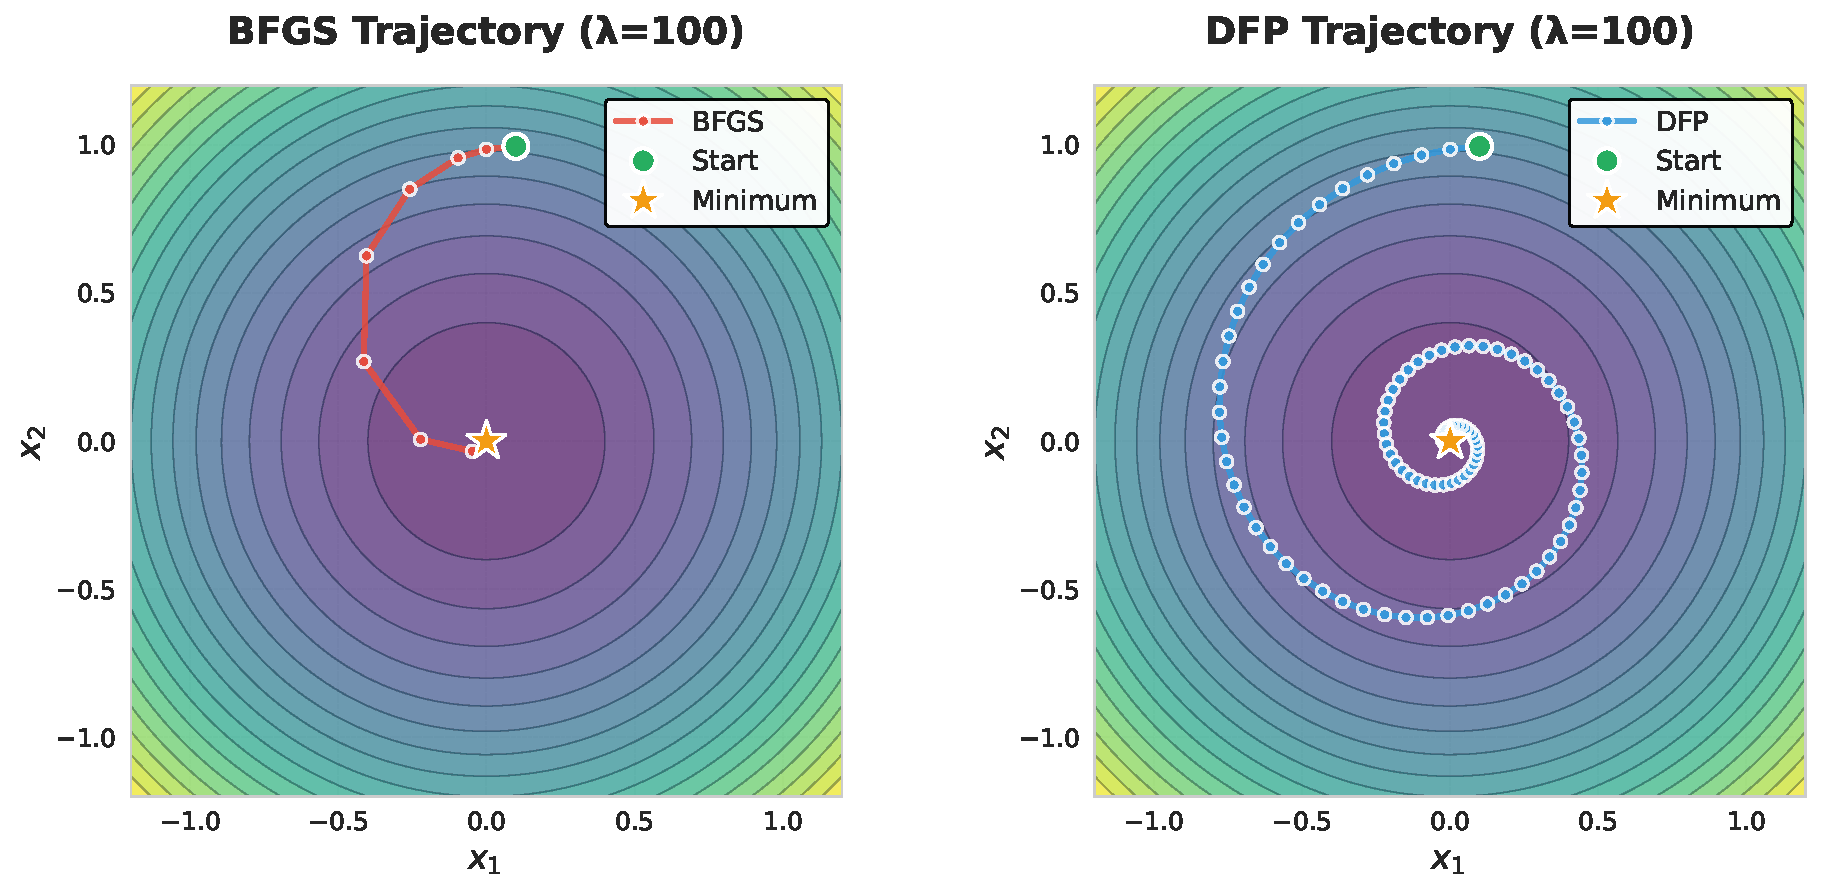
\includegraphics[width=\textwidth]{../imgs/quasi_newton/bfgs_vs_dfp_100.pdf}
    \caption{Iterative trajectories for BFGS and DFP methods when $\lambda_1 = 100$. BFGS converges in 10 iterations while DFP requires 107 iterations, showing BFGS's superior efficiency for large eigenvalue errors.}
    \label{fig:bfgs_dfp_100}
\end{figure}

\begin{figure}[t]
    \centering
    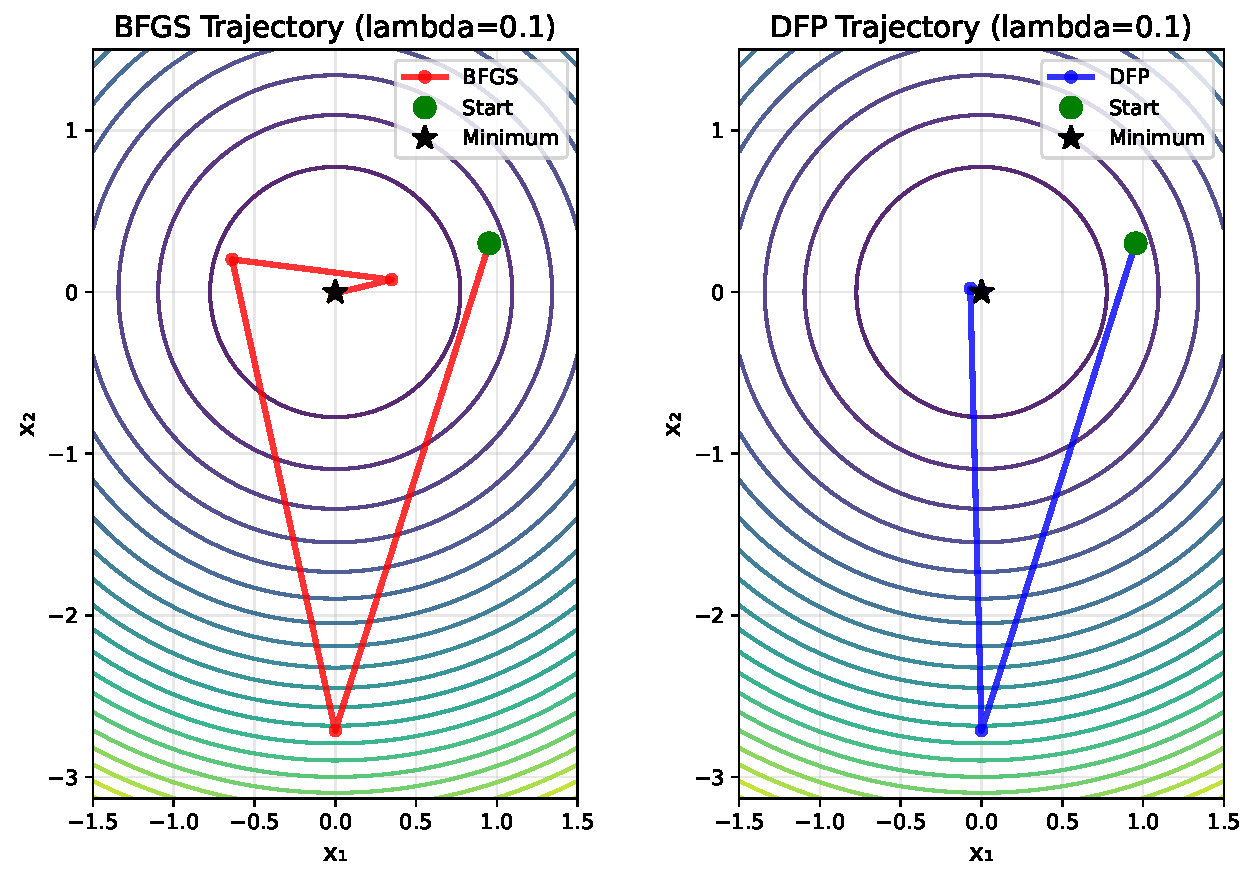
\includegraphics[width=\textwidth]{../imgs/quasi_newton/bfgs_vs_dfp_0.1.pdf}
    \caption{Iterative trajectories for BFGS and DFP methods when $\lambda_1 = 0.1$. Both methods converge quickly, with DFP slightly faster than BFGS, demonstrating the symmetric behavior when eigenvalues are underestimated.}
    \label{fig:bfgs_dfp_0p1}
\end{figure}

\subsubsection{Analysis and Discussion}

The numerical results reveal a striking asymmetry between BFGS and DFP.
When $\lambda_1 > 1$ (i.e., the initial Hessian approximation overestimates the true Hessian curvature), BFGS demonstrates significantly better efficiency.
Conversely, when $\lambda_1 < 1$ (i.e., the initial Hessian approximation underestimates the true curvature), DFP performs slightly better than BFGS, though the difference is modest.
This trend reversal is predicted by the theoretical symmetry between the two methods, but the magnitude of the difference is notable.

\paragraph{Asymmetry in Hessian Correction}

The asymmetry of the performance arises from a fundamental difference in how these two methods correct erroneous eigenvalues.
The core insight is that correcting erroneously large eigenvalues is more critical than correcting erroneously small ones.

When a Hessian eigenvalue is overestimated, the algorithm takes steps that are too conservative, resulting in slow progress toward the minimum. Correcting such errors requires the update formula to reduce these large eigenvalues toward one.
The BFGS update is highly effective at this task.

In contrast, when a Hessian eigenvalue is underestimated, the algorithm takes steps that are slightly too aggressive, but the error is self-correcting.
Subsequent gradient computations provide information that helps refine the approximation.
Thus, correcting underestimated eigenvalues is inherently easier and requires fewer iterations.

The DFP update struggles with large eigenvalues.
In the worst case, it can reduce a large eigenvalue by only a small amount per iteration, potentially requiring as many iterations as the magnitude of the eigenvalue itself.
This explains why DFP's performance degrades catastrophically as $\lambda_1$ increases beyond one.

\paragraph{Practical Implications}

These findings provide strong empirical justification for the widespread practical preference for BFGS over DFP.
The analysis of Powell's simple quadratic problem yields deep insights about quasi-Newton methods' behavior far from the solution, where most computational effort is expended.
The superior efficiency of BFGS in correcting erroneous Hessian approximations makes it the algorithm of choice for robust and efficient unconstrained optimization.

\subsection{Limited Memory BFGS (L-BFGS)}

Limited-memory quasi-Newton methods extend classical quasi-Newton methods to large-scale optimization problems.
In standard quasi-Newton methods, the approximate Hessian or inverse Hessian matrix is stored and updated as a dense matrix, requiring $\order{n^2}$ memory for $n$ variables.

The L-BFGS method \citep{liuLimitedMemoryBFGS1989a}, which is based on the BFGS update, avoids storing the full matrix explicitly.
Instead, it maintains only the most recent $m$ vector pairs $\{(s_i,y_i)\}$.
This reduces the storage requirement to $\order{nm}$, which is a dramatic improvement when $m$ is a small constant (typically $m\le 10$).

Throughout this subsection, we work with a finite sequence of matrices
\begin{equation*}
    H_0, H_1, \dots, H_m,
\end{equation*}
where $H_\ell$ denotes the inverse Hessian approximation obtained after $\ell$ BFGS updates applied to a given initial matrix $H_0$.
Note that this is not the same as the iterates in an optimization algorithm. Here, we focus solely on the structure of the BFGS updates.

\subsubsection{Compact Representation of \texorpdfstring{$H_m$}{Hm}}

Let $\{(s_i,y_i)\}_{i=0}^{m-1}$ be the stored correction pairs, and define
\begin{equation}\label{eq:rho-V-def}
    \rho_i = \frac{1}{y_i^\top s_i}, \qquad
    V_i = I - \rho_i y_i s_i^\top.
\end{equation}
From \cref{eq:Hk_rank}, the BFGS update for the inverse Hessian can be expressed as
\begin{equation}\label{eq:Hk-bfgs-rank}
    H_{i+1} = V_i^\top H_i V_i + \rho_i s_i s_i^\top,
\end{equation}
for $i = 0,\dots,m-1$.
By recursively expanding this relation, we obtain the compact representation
\begin{equation}\label{eq:Hm-compact}
    H_m
    =
    V_{m-1}^\top \cdots V_0^\top H_0 V_0 \cdots V_{m-1}
    +
    \sum_{j=0}^{m-1}
    (V_{m-1}^\top \cdots V_{j+1}^\top)
    \rho_j s_j s_j^\top
    (V_{j+1} \cdots V_{m-1}),
\end{equation}
where $H_0$ denotes the chosen initial inverse Hessian approximation, typically a scaled identity matrix.

\subsubsection{Two-Loop Recursion}

The compact representation above can be applied to any vector $q$ without explicitly forming $H_m$.
Let $r = H_m q$.
Exploiting the associative structure of the matrix products, this operation can be carried out using two short loops of length $m$, leading to the well-known L-BFGS two-loop recursion~\citep[Algorithm 7.4]{nocedal1999numerical}. The pseudocode is provided in \cref{alg:two-loop-recursion}.
This algorithm requires $\order{md}$ arithmetic operations and $\order{md}$ storage, where $d$ denotes the problem dimension.

\DontPrintSemicolon
\begin{algorithm}[t]
    \caption{L-BFGS Two-Loop Recursion for $r = H_m q$ \citep[Algorithm 7.4]{nocedal1999numerical}}
    \label{alg:two-loop-recursion}
    \KwIn{$q$, stored pairs $\{(s_i, y_i)\}_{i=0}^{m-1}$, initial matrix $H_0$}
    \KwOut{$r = H_m q$}
    \For{$i = m-1, m-2, \dots, 0$}{
        $\rho_i \gets 1/(y_i^\top s_i)$\;
        $\alpha_i \gets \rho_i s_i^\top q$\;
        $q \gets q - \alpha_i y_i$\;
    }
    $r \gets H_0 q$\;
    \For{$i = 0, \dots, m-1$}{
        $\beta_i \gets \rho_i y_i^\top r$\;
        $r \gets r + s_i (\alpha_i - \beta_i)$\;
    }
    \Return $r$\;
\end{algorithm}

Now, we verify that the output of \cref{alg:two-loop-recursion} indeed computes $r = H_m q$.
\begin{proposition}
    The output of the two-loop recursion \cref{alg:two-loop-recursion} satisfies $r = H_m q$.
\end{proposition}
\begin{proof}
    In the backward recursion, for $i = m-1, m-2, \dots, 0$, from the input vector $q^{(m)} \coloneqq q$, the algorithm computes
    \begin{equation}
        \alpha_i   = \rho_i s_i^\top q^{(i+1)}, \qquad
        q^{(i)} \coloneqq q^{(i+1)} - \alpha_i y_i.
    \end{equation}
    % Using the definition of $V_i$ and $\alpha_i$, we have
    Substituting the definition of $\alpha_i$ and using \cref{eq:rho-V-def}, we find
    \begin{equation*}
        q^{(i)} = q^{(i+1)} - \rho_i \qty(s_i^\top q^{(i+1)}) y_i = \qty(I - \rho_i y_i s_i^\top) q^{(i+1)} = V_i q^{(i+1)}.
    \end{equation*}
    Thus, for all $i = 0, 1, \dots, m-1$, we have
    \begin{equation*}
        q^{(i)} = V_i V_{i+1} \cdots V_{m-1} q.
    \end{equation*}
    Then, the algorithm applies the initial inverse Hessian approximation:
    \begin{equation*}
        r^{(0)} = H_0 q^{(0)} = H_0 V_0 V_1 \cdots V_{m-1} q.
    \end{equation*}
    Next, for $i = 0, 1, \dots, m-1$, the forward recursion computes
    \begin{equation*}
        \beta_i     = \rho_i y_i^\top r^{(i)}, \qquad
        r^{(i+1)}   = r^{(i)} + s_i \qty(\alpha_i - \beta_i).
    \end{equation*}
    Substituting the definitions of $\alpha_i$, $\beta_i$, and $q^{(i+1)}$, we have
    \begin{align*}
        r^{(i+1)}
         & =
        r^{(i)} + \rho_i s_i s_i^\top \qty(V_{i+1} V_{i+2} \cdots V_{m-1}) q - \rho_i s_i y_i^\top r^{(i)}     \\
         & = \qty(I- \rho_i y_i s_i^\top) r^{(i)} + \rho_i s_i s_i^\top \qty(V_{i+1} V_{i+2} \cdots V_{m-1}) q \\
         & =
        V_i^\top r^{(i)}
        +
        \rho_i s_i s_i^\top
        \qty(V_{i+1} V_{i+2} \cdots V_{m-1}) q.
    \end{align*}
    By recursively expanding this relation from the initial value $r^{(0)} = H_0 q^{(0)}$, we obtain
    \begin{equation}
        r^{(m)}
        =
        V_{m-1}^\top \cdots V_0^\top H_0 V_0 \cdots V_{m-1} q
        +
        \sum_{j=0}^{m-1}
        (V_{m-1}^\top \cdots V_{j+1}^\top)
        \rho_j s_j s_j^\top
        (V_{j+1} \cdots V_{m-1}) q,
    \end{equation}
    which matches the compact representation of $H_m$ in \cref{eq:Hm-compact} applied to $q$, completing the proof.
\end{proof}

Thus, the two-loop recursion exactly evaluates the action of $H_m$ on a vector while avoiding explicit matrix construction, achieving both mathematical rigor and computational efficiency.

\subsubsection{Initial Step Size}

A crucial component of the L-BFGS method is the choice of the initial matrix $H_0$.
A widely used and well-justified option is a scaled identity,
\begin{equation}
    H_0 = \gamma I,
\end{equation}
where the scaling parameter is chosen as
\begin{equation}
    \gamma = \frac{s_{m-1}^\top y_{m-1}}{y_{m-1}^\top y_{m-1}}.
    \label{eq:gamma_k_initial}
\end{equation}
This choice is motivated by the relationship between the approximate inverse Hessian and the local curvature of the objective function \citep{liuLimitedMemoryBFGS1989a,shannoMatrixConditioningNonlinear1978}.
To justify this scaling, assume that the objective function $f$ is twice continuously differentiable and consider the mean Hessian along the most recent step:
\begin{equation}
    \bar{G}
    =
    \int_0^1 \nabla^2 f(x + \tau s_{m-1}) \dd \tau ,
\end{equation}
where $s_{m-1}$ denotes the most recent displacement.
By the mean value theorem,
\begin{equation*}
    y_{m-1}
    =
    \nabla f(x+s_{m-1}) - \nabla f(x)
    =
    \bar{G} s_{m-1}.
\end{equation*}
Using this relation, the scaling factor can be written as
\begin{equation}
    \frac{s_{m-1}^\top y_{m-1}}{y_{m-1}^\top y_{m-1}}
    =
    \frac{(\bar{G}^{1/2} s_{m-1})^\top (\bar{G}^{1/2} s_{m-1})}
    {(\bar{G}^{1/2} s_{m-1})^\top \bar{G} (\bar{G}^{1/2} s_{m-1})},
    \label{eq:rayleigh_form}
\end{equation}
which is a Rayleigh quotient.
If $\bar{G}^{1/2} s_{m-1}$ happens to be an eigenvector of $\bar{G}$, then the reciprocal of this quantity equals the corresponding eigenvalue.

Moreover, the choice \eqref{eq:gamma_k_initial} coincides with the short step size of the Barzilai--Borwein method \citep{barzilaiTwoPointStepSize1988}, highlighting a close connection between L-BFGS initialization and classical step-length selection strategies.
This observation further supports the effectiveness of the scaled-identity initialization in practice.

\ifSubfilesClassLoaded{
    \bibliographystyle{plainnat}
    \bibliography{../L-BFGS.bib}
}{}

\end{document}
